\documentclass[conference]{IEEEtran}
\IEEEoverridecommandlockouts
\usepackage{cite}
\usepackage{amsmath,amssymb,amsfonts}
\usepackage{algorithmic}
\usepackage{graphicx}
\usepackage{textcomp}
\usepackage{xcolor}
\usepackage{booktabs}
\usepackage{array}
\usepackage{url}
\def\BibTeX{{\rm B\kern-.05em{\sc i\kern-.025em b}\kern-.08em
    T\kern-.1667em\lower.7ex\hbox{E}\kern-.125emX}}

\begin{document}

\title{Checkpoint Charlie: Final Report on Layered BGP Path Security from Selective Verification to ASPA/OTC/GNN Fusion}

\author{
\IEEEauthorblockN{Tanmay Parihar}
\IEEEauthorblockA{\textit{School of Electrical Engineering} \\
\textit{Manipal Institute of Technology}\\
Manipal, India \\
tanmay4.mitmpl2023@learner.manipal.edu}
\and
\IEEEauthorblockN{Ayush Shetty}
\IEEEauthorblockA{\textit{School of Electrical Engineering} \\
\textit{Manipal Institute of Technology}\\
Manipal, India \\
ayush14.mitmpl2023@learner.manipal.edu}
}

\maketitle

\begin{abstract}
Border Gateway Protocol (BGP) remains vulnerable because route announcements are largely trust-based. Our project began with the same core question stated in the synopsis: can we achieve strong security between lightweight origin validation (RPKI) and expensive full-path cryptographic validation (BGPsec)? We implemented and evaluated a complete layered framework in three stages: (i) selective-hop path verification plus statistical anomaly detection, (ii) incremental Delta Trust verification, and (iii) an enhanced stack with route-leak modeling, ASPA, OTC, graph-based anomaly detection, and probabilistic signal fusion. The final system was evaluated on synthetic AS-level topologies with mixed legitimate and malicious traffic, including origin hijack, path shortening, path fabrication, and three route-leak classes. Key findings include: selective+anomaly reached 98.09\% detection in the baseline phase with low false positives; Delta Trust matched BGPsec detection (99.05\%) at lower modeled cost; and in the enhanced route-leak-inclusive phase, OTC achieved perfect leak-type detection while Path Plausibility achieved AUC 0.9901 with zero false positives at its operating threshold. These results show that practical layered defenses can significantly improve BGP security without depending on full-path cryptographic verification alone.
\end{abstract}

\begin{IEEEkeywords}
BGP security, RPKI, BGPsec, selective hop verification, anomaly detection, route leaks, ASPA, OTC, graph neural networks
\end{IEEEkeywords}

\section{Introduction}
BGP controls inter-domain routing among tens of thousands of autonomous systems (ASes). Its default trust model allows malicious or misconfigured ASes to advertise incorrect reachability, enabling traffic hijacks, route leaks, and path manipulation. The YouTube hijack incident and repeated large-scale route leaks demonstrate that this is an operational problem, not only a theoretical one.

Our initial synopsis proposed two practical middle-ground defenses between RPKI and BGPsec: selective hop verification and statistical anomaly detection. During execution, the project evolved into a broader layered framework to include incremental validation and modern route-leak-focused techniques. This final report retains the original objective and reports all phases of implementation and findings.

\section{Problem Formulation and Project Objectives}
The central problem is the security-cost trade-off:
\begin{itemize}
\item RPKI is efficient but only validates origin-prefix binding.
\item BGPsec validates full path integrity but incurs high cryptographic overhead.
\end{itemize}

We formulated five concrete objectives:
\begin{enumerate}
\item Build a reproducible simulation framework for AS topology, route generation, and attack injection.
\item Quantify security-cost trade-offs for selective path validation positions.
\item Add low-cost statistical and incremental trust methods to improve practical deployability.
\item Extend the threat model to route leaks and evaluate modern leak-mitigation techniques (ASPA, OTC).
\item Fuse heterogeneous security signals into a single decision engine and evaluate with ROC/AUC analysis.
\end{enumerate}

\section{Background and Related Work}
\subsection{RPKI and BGPsec}
RPKI (RFC 6480) provides cryptographic authorization for route origins. It is practical but origin-only. BGPsec (RFC 8205) provides path-level cryptographic protection but is computationally expensive and operationally challenging to deploy.

\subsection{Route Leak Mitigation}
Route leaks are now a primary operational concern. RFC 9234 introduces BGP Roles and the OTC (Only-To-Customer) attribute for leak prevention and detection. ASPA is an emerging SIDROPS mechanism to validate provider authorization across AS\_PATH segments.

\subsection{Data-Driven and Graph-Based Detection}
Anomaly detection complements cryptographic mechanisms by identifying suspicious behavior patterns. Recent work indicates graph-aware approaches can improve anomaly discrimination by using topology structure.

\section{System Architecture and Methodology}
\subsection{Simulation Pipeline}
The framework builds a Barabasi-Albert AS graph, assigns AS tiers and relationships, generates legitimate routes, injects attacks, runs validators, and computes metrics/plots. We retained the original baseline pipeline and added new modules in separate files (no modifications to legacy files).

\subsection{Topology and Traffic Model}
The topology generator assigns customer-provider and peer-peer roles and checks valley-free consistency. Route generation uses shortest AS paths with path-length bounds for realistic synthetic traffic.

\subsection{Attack Model}
Original attack set:
\begin{itemize}
\item Origin hijack
\item Path shortening
\item Path fabrication
\end{itemize}

Enhanced attack set:
\begin{itemize}
\item Route leak Type-1: full-prefix leak
\item Route leak Type-2: lateral leak
\item Route leak Type-3: intentional strategic leak
\end{itemize}

\subsection{Validation Stack}
The implemented validator set includes:
\begin{itemize}
\item \textbf{RPKI}: origin validation.
\item \textbf{Selective Hop}: configurable hop-position verification.
\item \textbf{BGPsec model}: full-hop verification.
\item \textbf{Anomaly Detector}: statistical feature scoring (path length, origin changes, valley-free checks, unseen ASes, loops).
\item \textbf{Delta Trust}: cache-based incremental edge verification.
\item \textbf{ASPA}: provider authorization checks with partial deployment parameter.
\item \textbf{OTC}: route-leak detection based on OTC signal and relationship direction.
\item \textbf{GNN Anomaly Detector}: topology-aware message passing for anomaly scoring.
\item \textbf{Path Plausibility}: weighted probabilistic fusion of all signal classes.
\end{itemize}

\subsection{Metrics}
We use:
\begin{align}
\text{Detection Rate} &= \frac{\text{Detected Attacks}}{\text{Total Attacks}} \\
\text{False Positive Rate} &= \frac{\text{Legitimate Rejected}}{\text{Total Legitimate}} \\
\text{Security-Cost Ratio} &= \frac{\text{Detection Rate}}{\text{Average Time (ms)}}
\end{align}

Timing values are model-based (hash lookup and cryptographic-operation constants), used for relative comparison across validators.

\section{Implementation Evolution}
\subsection{Phase I: Baseline (Original Scope)}
Files: \texttt{main.py}, baseline validators in \texttt{src/validators}. This phase delivered the original synopsis goals: selective validation and anomaly detection trade-off analysis.

\subsection{Phase II: Incremental Trust}
Files: \texttt{src/validators/delta\_trust.py}, \texttt{delta\_main.py}, \texttt{delta\_combined\_main.py}. Delta Trust introduced edge-cache reuse, reducing repeated cryptographic work.

\subsection{Phase III: Enhanced Framework}
Files added in this phase:
\begin{itemize}
\item \texttt{enhanced\_main.py}
\item \texttt{src/validators/aspa.py}
\item \texttt{src/validators/otc.py}
\item \texttt{src/validators/gnn\_anomaly.py}
\item \texttt{src/validators/path\_plausibility.py}
\item \texttt{src/attacks/route\_leak.py}
\item \texttt{src/enhanced\_visualization.py}
\end{itemize}

\section{Experimental Setup}
\subsection{Runs and Artifacts}
We report from four experiment sets:
\begin{itemize}
\item \texttt{results/} (baseline, 4,984 announcements)
\item \texttt{results\_delta/} (with Delta Trust, 19,954 announcements)
\item \texttt{results\_delta\_combined/} (Delta + original combined, 19,954 announcements)
\item \texttt{results\_enhanced/} (enhanced stack + route leaks, 20,000 announcements)
\end{itemize}

\subsection{Evaluation Outputs}
Each run exports:
\begin{itemize}
\item \texttt{summary.csv}, \texttt{attack\_breakdown.csv}
\item cost-security plots and breakdown figures
\item enhanced plots: ASPA sweep, leak heatmap, fusion ablation, radar, ROC curves
\end{itemize}

\section{Results and Analysis}
\subsection{Phase-Wise Quantitative Summary}
Table~\ref{tab:phase_summary} summarizes representative results retained from each project stage.

\begin{table*}[t]
\caption{Representative Results Across Project Phases}
\label{tab:phase_summary}
\centering
\begin{tabular}{@{}l l c c c c@{}}
\toprule
\textbf{Phase} & \textbf{Validator} & \textbf{Detection Rate} & \textbf{FPR} & \textbf{Avg Time (ms)} & \textbf{Security-Cost Ratio} \\
\midrule
Baseline (\texttt{results}) & RPKI & 0.1894 & 0.0000 & 0.230606 & 0.8212 \\
Baseline (\texttt{results}) & Origin + 1st + Last & 0.9496 & 0.0000 & 1.440409 & 0.6593 \\
Baseline (\texttt{results}) & BGPsec (Full Path) & 0.9837 & 0.0000 & 1.732243 & 0.5678 \\
Baseline (\texttt{results}) & Anomaly Detector & 0.7616 & 0.0000 & 0.050000 & 15.2316 \\
Baseline (\texttt{results}) & Selective + Anomaly & 0.9809 & 0.0000 & 1.490409 & 0.6582 \\
\midrule
Delta (\texttt{results\_delta}) & BGPsec (Full Path) & 0.9905 & 0.0000 & 1.858049 & 0.5331 \\
Delta (\texttt{results\_delta}) & Delta Trust & 0.9905 & 0.0000 & 1.474468 & 0.6718 \\
Delta Combined (\texttt{results\_delta\_combined}) & Delta + Selective + Anomaly & 0.9919 & 0.0016 & 2.984677 & 0.3323 \\
\midrule
Enhanced (\texttt{results\_enhanced}) & ASPA (50\%) & 0.6863 & 0.0000 & 0.038142 & 17.9944 \\
Enhanced (\texttt{results\_enhanced}) & OTC (50\%) & 0.3497 & 0.0000 & 0.015870 & 22.0332 \\
Enhanced (\texttt{results\_enhanced}) & GNN Anomaly Detector & 0.2457 & 0.0300 & 1.500000 & 0.1638 \\
Enhanced (\texttt{results\_enhanced}) & Selective + Anomaly & 0.8520 & 0.0016 & 1.517800 & 0.5613 \\
Enhanced (\texttt{results\_enhanced}) & Path Plausibility & 0.7547 & 0.0000 & 4.843812 & 0.1558 \\
\bottomrule
\end{tabular}
\end{table*}

\subsection{Baseline Insights (Original Thesis Validation)}
The original synopsis hypothesis was that selective hop checks can provide near-BGPsec security at lower cost. This was validated in \texttt{results/}: ``Origin + 1st + Last'' reached 94.96\% detection versus 98.37\% for full-path BGPsec, while requiring fewer modeled cryptographic operations. The statistical anomaly detector contributed a very favorable efficiency profile (15.23 security-cost ratio), and the combined selective+anomaly strategy reached 98.09\%.

\subsection{Delta Trust Contribution}
Delta Trust preserved high security while lowering cost on repeated-prefix traffic. In \texttt{results\_delta/}, Delta Trust matched BGPsec detection (99.05\%) with lower average modeled time (1.474468 ms vs 1.858049 ms), improving efficiency for stable routing states.

\subsection{Enhanced Route-Leak-Centric Findings}
In \texttt{results\_enhanced/}, the attack set includes route leaks, making the evaluation materially harder and more realistic. This changed rankings compared to baseline-only path-manipulation experiments:
\begin{itemize}
\item Selective+Anomaly remained the strongest practical detector at 85.20\%.
\item OTC showed perfect per-type leak detection (Type-1/2/3 all 1.0) in attack-type breakdown.
\item ASPA/Delta/BGPsec had identical overall detection in this run because they were driven by similar adjacency-based checks in the implemented model.
\item GNN had low thresholded operating-point detection (24.57\%) but still yielded strong ROC AUC (0.8663), showing useful ranking capability despite weak default threshold calibration.
\item Path Plausibility reached AUC 0.9901 with zero FPR at its configured threshold.
\end{itemize}

\subsection{Leak-Type Breakdown}
Table~\ref{tab:leak_breakdown} reports route-leak detection for selected validators from \texttt{results\_enhanced/attack\_breakdown.csv}.

\begin{table}[t]
\caption{Route-Leak Detection Rates (Enhanced Run)}
\label{tab:leak_breakdown}
\centering
\begin{tabular}{@{}lccc@{}}
\toprule
\textbf{Validator} & \textbf{Type-1} & \textbf{Type-2} & \textbf{Type-3} \\
\midrule
RPKI & 0.0000 & 0.0000 & 0.0000 \\
BGPsec (Full Path) & 0.0000 & 0.0000 & 0.6462 \\
ASPA (50\%) & 0.0000 & 0.0000 & 0.6462 \\
OTC (50\%) & 1.0000 & 1.0000 & 1.0000 \\
Anomaly Detector & 0.4502 & 0.8342 & 0.1385 \\
Path Plausibility & 0.2879 & 0.1301 & 0.7436 \\
\bottomrule
\end{tabular}
\end{table}

\subsection{Fusion Ablation and ROC}
The enhanced fusion analysis produced two notable outputs:
\begin{itemize}
\item \textbf{ROC:} AUC values were 0.8663 (GNN Anomaly Detector) and 0.9901 (Path Plausibility).
\item \textbf{Ablation:} removing GNN reduced fusion detection from 0.7579 to 0.6852, indicating that GNN ranking signal contributes significant marginal value to fusion.
\end{itemize}

At the same time, ``No ASPA'' outperformed ``All signals'' in one ablation run, indicating calibration mismatch among fused signals in the current implementation. This is an important engineering outcome and directly informs future tuning work.

\section{Figures}
\begin{figure}[t]
\centering
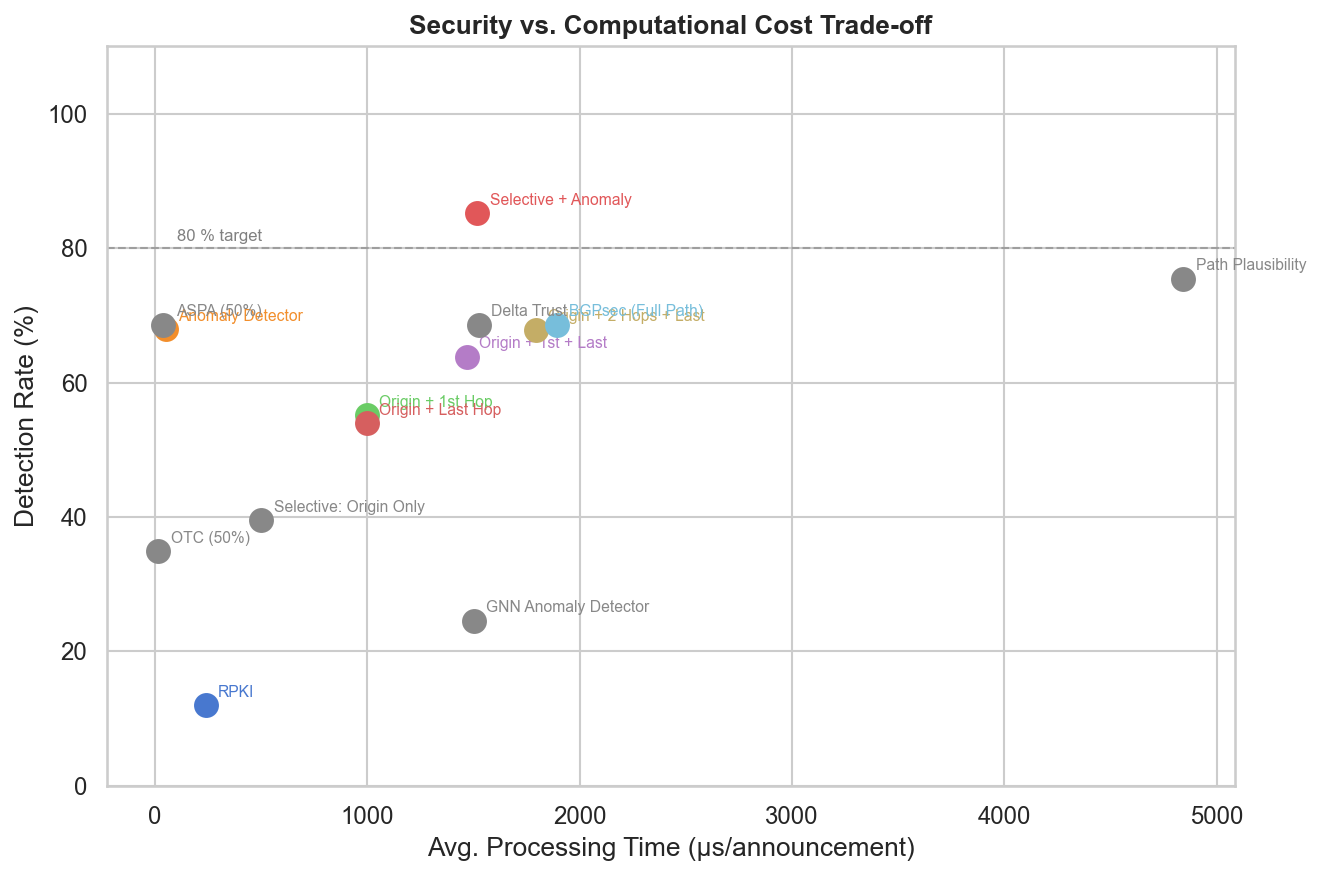
\includegraphics[width=\linewidth]{results_enhanced/security_cost_tradeoff.png}
\caption{Enhanced run: detection versus modeled processing cost.}
\label{fig:enhanced_tradeoff}
\end{figure}

\begin{figure}[t]
\centering
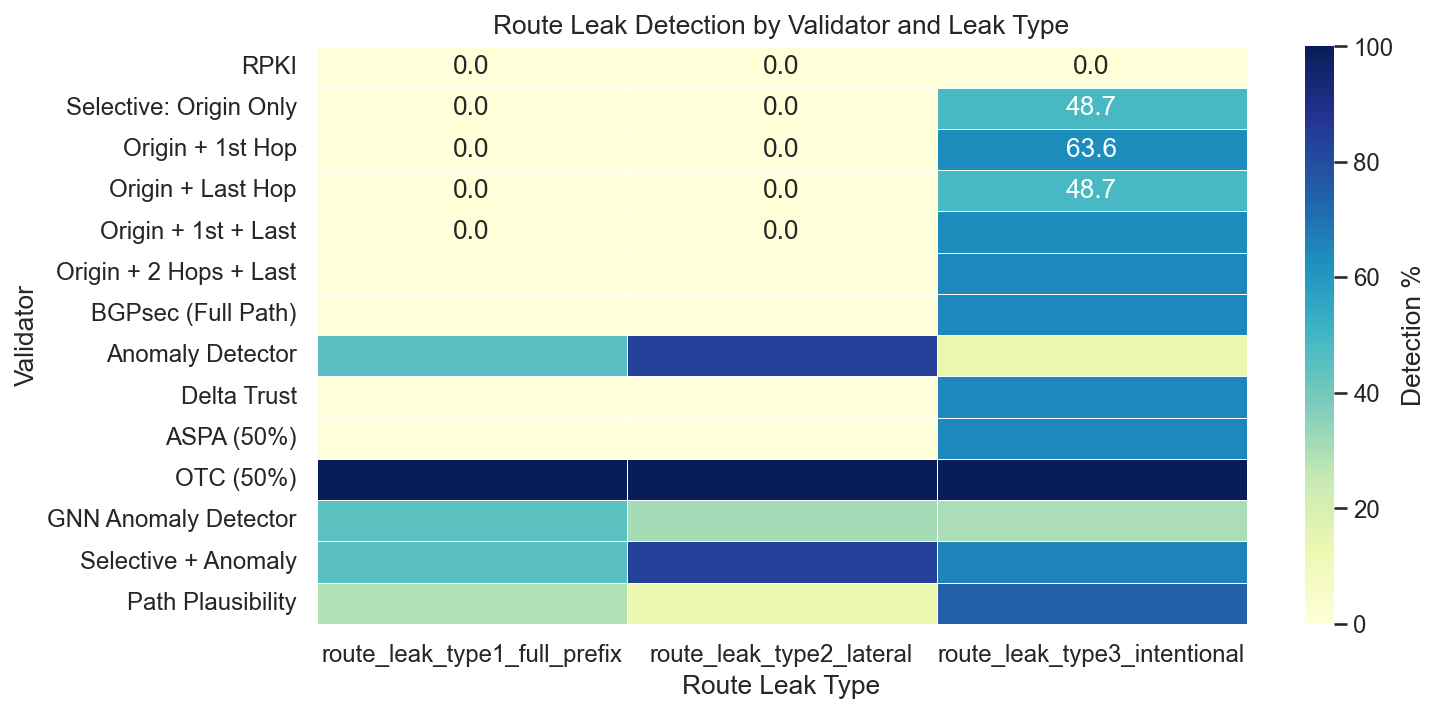
\includegraphics[width=\linewidth]{results_enhanced/route_leak_detection_heatmap.png}
\caption{Enhanced run: route-leak subtype detection heatmap.}
\label{fig:enhanced_leak_heatmap}
\end{figure}

\begin{figure}[t]
\centering
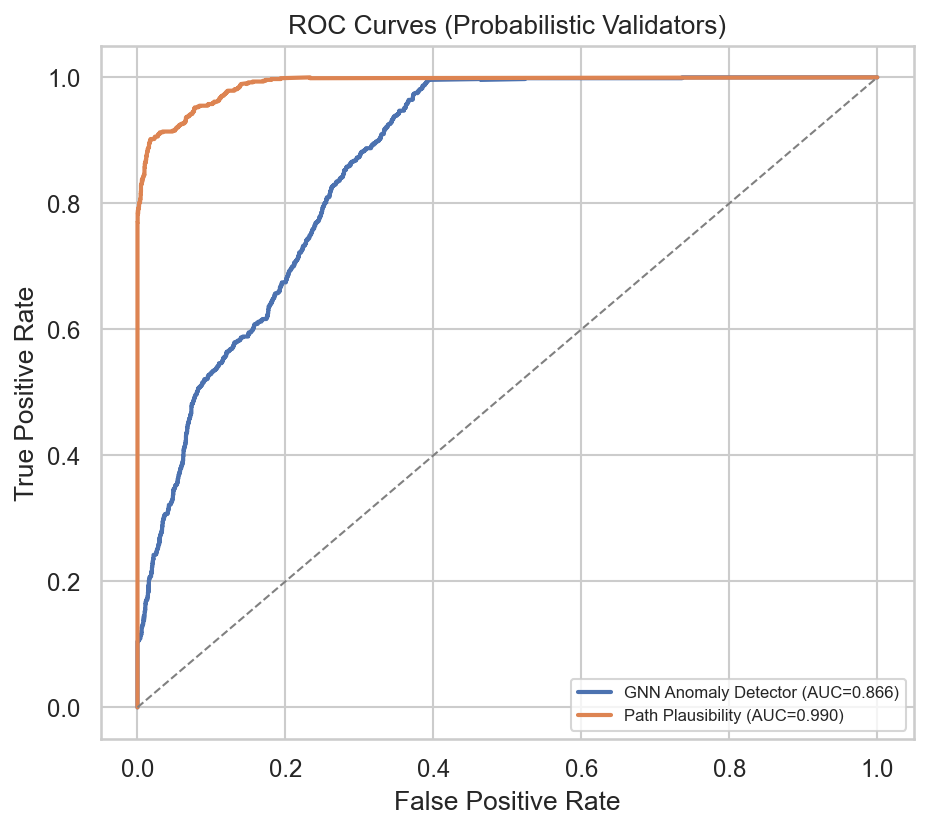
\includegraphics[width=\linewidth]{results_enhanced/roc_curves.png}
\caption{ROC curves for probabilistic validators in enhanced evaluation.}
\label{fig:enhanced_roc}
\end{figure}

\section{Discussion}
The project evolution confirms the original thesis and adds practical depth:
\begin{itemize}
\item Selective cryptographic verification is a robust middle point between RPKI and BGPsec for non-leak path attacks.
\item Statistical/ML methods are not replacements for cryptographic checks, but materially increase coverage in combined operation.
\item Route leaks require explicit modeling and dedicated controls; OTC is highly effective in this implementation.
\item Signal fusion can produce very strong ranking performance (AUC), but threshold and weight calibration are critical to convert ranking strength into best operating-point detection.
\end{itemize}

\section{Limitations}
\begin{itemize}
\item Timing values are modeled and relative, not router hardware measurements.
\item The topology and traffic are synthetic; realism improves with public trace replay and control-plane event datasets.
\item ASPA and OTC implementations are simulation-oriented simplifications, not production protocol stacks.
\item GNN module uses lightweight message passing and thresholding; full supervised graph training and calibration were outside this submission scope.
\end{itemize}

\section{Conclusion and Future Work}
This project started from a selective-verification synopsis and matured into a complete layered BGP security framework. Baseline results validated that selective hop verification plus anomaly detection can approach BGPsec-level protection for many attacks. Delta Trust improved efficiency without sacrificing detection in stable-route scenarios. The enhanced framework added route-leak realism and modern defenses (ASPA, OTC, GNN, and probabilistic fusion), showing that no single mechanism is sufficient across all attack classes.

Future work will focus on (i) calibration and learning of fusion weights, (ii) stronger ASPA/OTC protocol-faithful modeling under partial deployment, (iii) real BGP trace integration, and (iv) hardware-aware timing validation for operational deployment planning.

\begin{thebibliography}{00}
\bibitem{b1} M. Lepinski and K. Sriram, ``BGPsec Protocol Specification,'' RFC 8205, Sep. 2017.
\bibitem{b2} M. Lepinski and S. Kent, ``An Infrastructure to Support Secure Internet Routing,'' RFC 6480, Feb. 2012.
\bibitem{b3} A. Azimov et al., ``Route Leak Prevention and Detection Using Roles in UPDATE and OPEN Messages,'' RFC 9234, Jun. 2022.
\bibitem{b4} SIDROPS WG, ``ASPA Verification,'' \textit{IETF Internet-Draft}, draft-ietf-sidrops-aspa-verification, 2025--2026.
\bibitem{b5} Y. Gilad et al., ``Are We There Yet? On RPKI's Deployment and Security,'' in \textit{Proc. NDSS}, 2017.
\bibitem{b6} K. Butler et al., ``A Survey of BGP Security Issues and Solutions,'' \textit{Proc. IEEE}, vol. 98, no. 1, pp. 100--122, 2010.
\bibitem{b7} K. Sriram et al., ``NIST SP 800-189 Rev.1 (Initial Public Draft): Resilient Interdomain Traffic Exchange,'' NIST, Jan. 2025.
\bibitem{b8} J. Furuness et al., ``Securing BGP ASAP: ASPA and Other Post-ROV Defenses,'' in \textit{Proc. NDSS}, 2025.
\bibitem{b9} A. Rahali et al., ``Unveiling the Potential of Graph Neural Networks for BGP Anomaly Detection,'' in \textit{Proc. ACM CoNEXT GNNet Workshop}, 2022.
\bibitem{b10} Checkpoint Charlie Project Repository, ``Simulation outputs and source code,'' 2026.
\end{thebibliography}

\end{document}
